\documentclass{article}
\usepackage{graphicx}
\usepackage{subfig}
\usepackage{amsmath}
\begin{document}
\section{Introduction}
\subsection{Motivation: CETD use new designed component, the formal security
analysis is not provided with the design}
Message authentication code(MAC) is a cryptographic system to protect the integrity of message transmitted between sender and receiver. If the content of message blocks are modified or external message blocks are injected, a secure MAC scheme should be eligible to examine the attacks. When using a MAC scheme to protect the integrity, message blocks are adopted to a MAC scheme as input and a short message block, called tag in majority of research works, is generated as output. The tag is concatenated to the input message blocks and this data-tag pair is used as unit in transmission. Early MAC schemes are symmetric-keyed, stateless(secrete key is the only resource of randomness in tag generation) and constructed with block cipher. As stateless MAC schemes suffer from replay attacks, MAC schemes using state information of message blocks protected as additional information in tag generation have been designed.

Hong, Guo and Hu\cite{cetd} introduced a cost-effective tag design for integrity protection, specially for embedded systems. The MAC scheme adopted is an stateful design constructed with two components: bit segments swap and block-level rotate shift. When generating a tag, a nonce generated by encrypting a tuple(message address, counter, random number) is used as additional input in processing the input data for swap and shift components. 
A security analysis of the MAC scheme adopted was provided by Hong et al. indicating that tag generated is random under brute-force attack. This evaluation procedure contains the following weakness:
\begin{itemize}
	\item The capability of the adversary is not depicted clearly
	\item The security result under each type of attack in the threat model is not provided
	\item The data processing components used in constructing the MAC scheme in cost-effective tag design are not cryptographic primitives, the security assumption of these components are unclear.
	\item The evaluation procedure does not belong to any common formal evaluation framework. The security result provided can not be used in comparison with the formal results from evaluation of other MAC schemes.
\end{itemize}
The tag design from Hong et al. showed  reduction of on-chip, performance and memory overhead. This cost advantage attracted us to research its security with a formal approach.
\subsection{Approach: Analysis the security of CETD with computational model}
In this article, we will show that from the viewpoint of computational model based security analysis, the secure block cipher used in generating nonce can not ensure the security of Cost-Effective Tag Design as a message authentication system under several attacks. To make this statement meaningful, we follow the well recognized security notions of message authentication system in computational model.
\subsection{Results: found security weakness, security optimization and results for optimized design }

\section{Preliminary: Formal Approaches of Security Analysis}
\paragraph{Threat Model of Data Integrity}
We use processor-memory system to explain the threat and protection on the integrity of message blocks in transmission. 
In the scenario of processor-memory architecture, data integrity refers to maintaining the data on the transmission outside the chip and stored on off-chip memory untampered. If the data stored on off-chip memory , or some external data injected to the system S, we can say that the data integrity of S is attacked. If the system S can not examine the tampered data or injected data, the attack is assumed to be successful. According to our knowledge, there are two aspects of attacks on data integrity:
\begin{enumerate}
	\item Introducing new content: The content of data in the system is modified, or data construct by the attacker is inserted to the system.
	\item Replacing data with valid copy: The data D in transmission or on the memory is replace with the following two types of copy: A copy of D at an old time point or a copy of other data from different memory address.
\end{enumerate}
\begin{figure}[htbp]
\centering
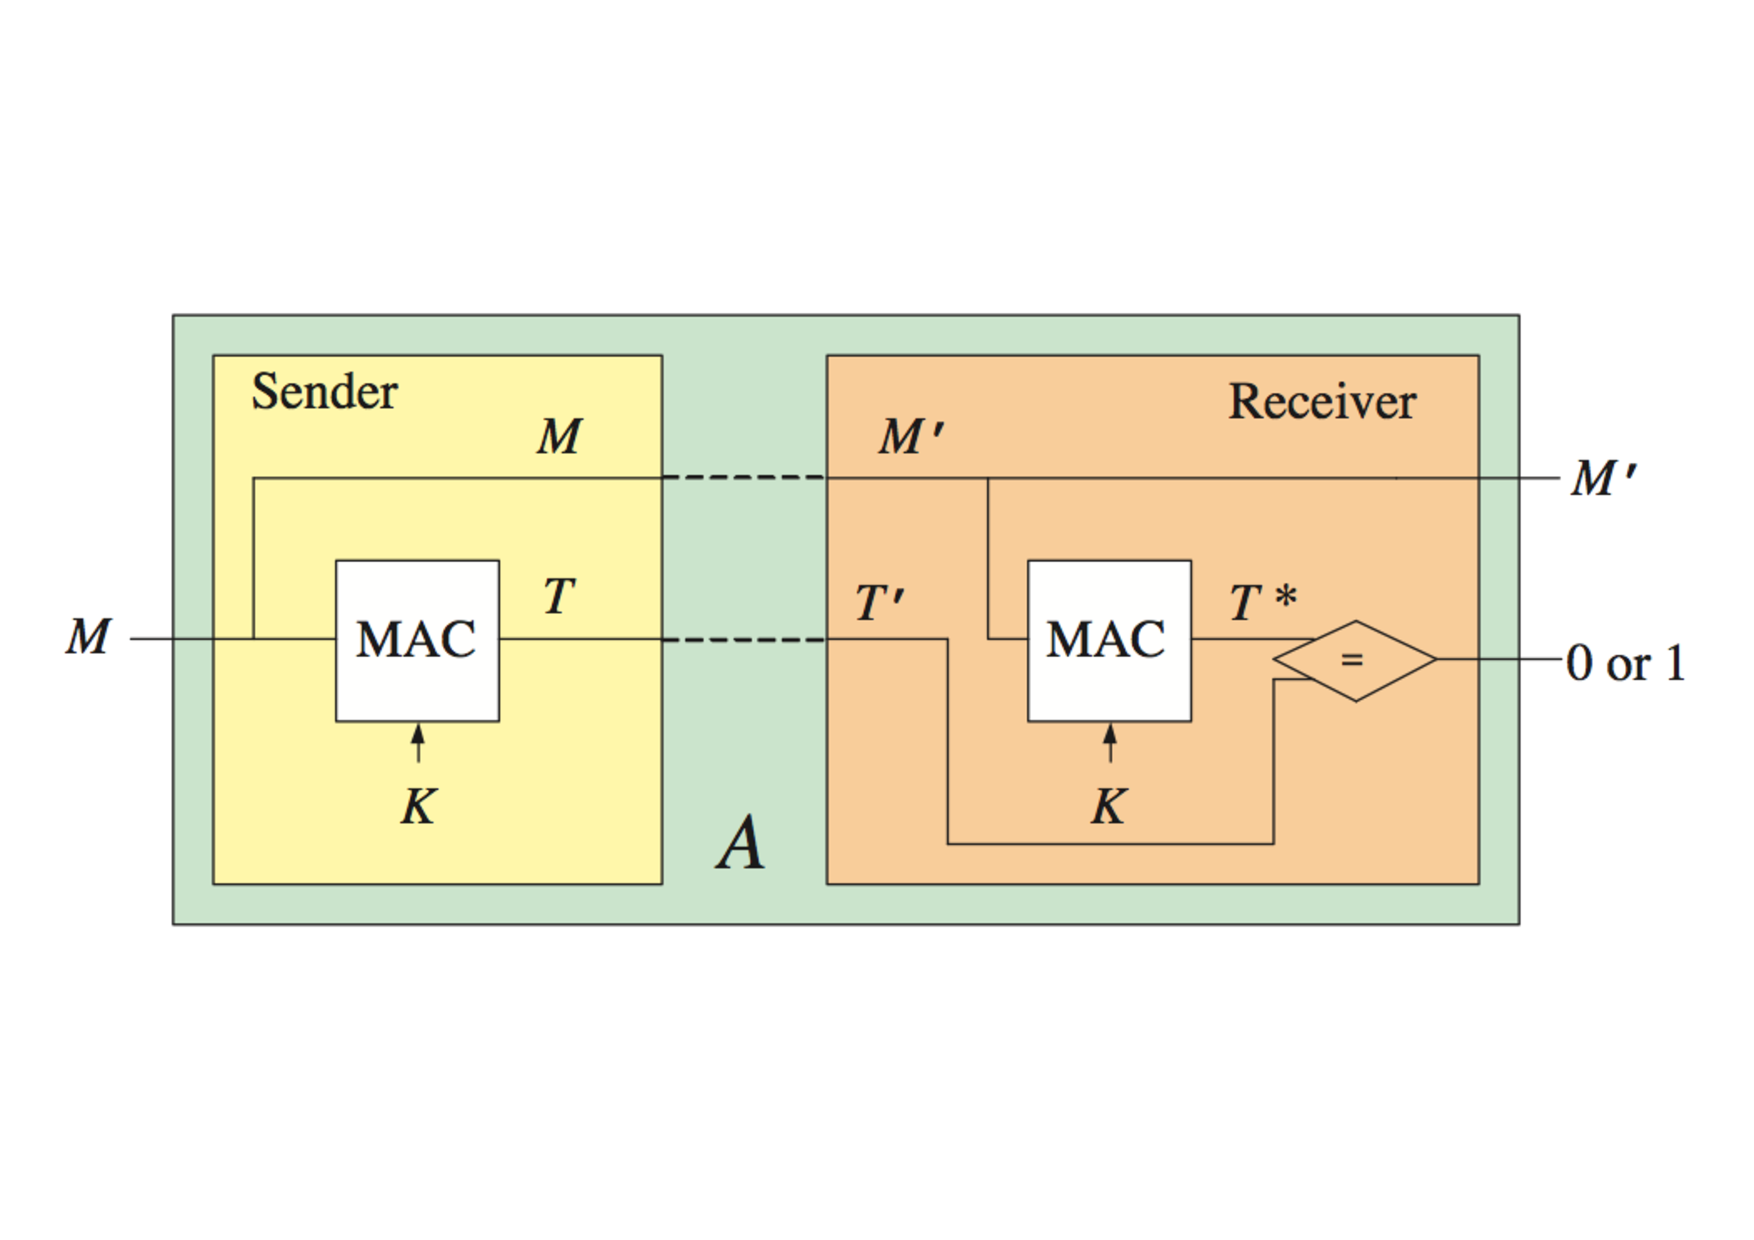
\includegraphics[scale=0.4]{./diagrams/MAC.pdf}
\caption{The Concept of Deterministic MAC Scheme}
\label{deterministic_mac }
\end{figure}

When the processor writes a data block D to the memory, MAC scheme computes a tag  and concatenate the tag withe data forming a data-tag pair. The data-tag pair is sent to off-chip memory for storage.
When the processor reads a data from memory, the data-pair is sent to the chip and to MAC scheme. Assume the data part is D and tag part is T1. MAC scheme compute a tag T2 using D T2 is compared with T1. If T1 is identical to T2, D is assumed to be untampered.
 Figure 3-b expresses the functionality of MAC scheme in integrity protection.
If the integrity of a processor-memory system is protected by MAC scheme, the possible attacks are:
\begin{enumerate}
	\item Modify the content of a data-tag pair
	\item Insert new data-tag pair
	\item Replace the content of a data-tag pair with a copy of data-tag pair from other address
	\item Replace the content of a data-tag pair with a copy of this pair in an old time point
\end{enumerate}
If a MAC scheme is capable to defend the 1st and 2nd attacks in the list, it should ensure that for any data block D, the tag is randomly assigned. If this scheme is capable to defend the 3rd and 4th attacks too, it should ensure for any two identical data blocks D1 and D2 that are written to memory on different time or to different addresses, their tags T1 and T2 should be randomly generated.

\subsection{Symbolic Model based Security Analysis}
Dolev and Yao introduced \cite{Dolev-Yao} a evaluation mechanism for analyzing the security of cryptographic protocol in
symbolic model(called formal methods in some research works). Each operation in the protocol analyzed is modeled to a term
algebra with strong security assumption. The security result of a protocol in
Dolev-Yao model has two possible value: secure with cryptographic primitive used
behaves like black box or an attack breaking the protocol exist.  
\paragraph{Symbolic Model Based Security Analysis on MAC Schemes}
In Dolev and Yao`s work, only framework of modeling encryption protocols was
introduced. The main weakness of Dolev-Yao model pointed by latter research
articles is that security assumption on the components used in the protocol is
too strong and unreal. The security result drawn with Dolev-Yao model can not
clearly indicate the security of a protocol in real application. In
\cite{symbolic-mac},
Backes, Pfitzmann and Waidner introduced an extension of Dolev-Yao framework to
support analyzing authentication systems such as digital signature and MAC
schemes. Another progress made by this extension is a bridge from symbolic model
to a result in computational model which represent the security of
authentication protocol in real world application.  Backes et al. analyzed the security of an authentication protocol
Kerberos with the framework in \cite{symbolic-kerberos}.

As pointed by Boldyreva and Kumar in \cite{computational-kerberos}, the weakness of the symbolic model based security
analysis of Kerberos from Backes et al. is the strong assumption of
cryptographic primitives used in Kerberos. This weakness represents the limitation
of existing symbolic model based security analysis approaches on authentication
systems: the authentication systems analyzed should be constructed with
cryptographic primitives meeting strong security assumptions. If the
authentication system analyzed is constructed with original designed components,
symbolic model based security analysis approaches can not be applied. 
Detailed survey of symbolic model based security analysis approaches can be
referred from \cite{symbolic-survey}.

\subsection{Computational Model based Security Analysis}
\subsubsection{Security Notion of MAC Schemes in Computational Model}
From the viewpoint of computational model, the security of a MAC scheme can be
broken if the resources, such as computation time, is unlimited for the
attacker, and AP system can always be broken at some time. Research works on
security analysis on MAC schemes try quantify the evaluation result under the assumption that the attack has limitation on computation resources.
\paragraph{The forgery attacks on MAC Schemes}
When attacking a MAC Scheme, the adversary try to send a pair(M,T) to the receiver to make VF$_k$(M,T)=1 while M did not originate with the legal sender. The fake pair(M$_f$,T$_f$) that makes VF$_k$(M$_f$,T$_f$)=1 is called a forgery from the adversary. A successful forgery attack indicates that the adversary has made a forgery. 
The purpose of a message authentication system is preventing the receiver to accept the message from unauthorized senders, such as an adversary. The quantitative property of a secure message authentication system is the low probability for an adversary to make a successful forgery attack with the limited resource.
\paragraph{Chosen-message attacks}
A strong type of attack that an adversary can conduct on the message authentication system is the adaptive chosen-message attack, marked as uf-cma. When doing uf-cma, the adversary chooses its own input message M and acquires the relative tag T. The adversary try to find the weakness in the design of message authentication system by analyzing the pairs(M,T) of his choice. The uf-cma provides the adversary with the most capability to succeed in the forgery attack. The probability that an adversary conducts a successful forgery attack after limited times of uf-cma is adopted as the basic quantitative security property of a message authentication in cryptography. This fact was also mentioned in \cite{Rogaway2011}.
\paragraph{The Security Notions of MAC schemes}
The formalised quantitative notion of the security of a MAC scheme was introduced by Bellare et al. in \cite{cbc1994}. This notion follows the security notion of digital signature introduced in \cite{signature}. The successful forgery on a MAC scheme from an adversary A is measured by a experiment called Forgery(MAC,A). In Forgery(MAC,A),  
the adversary A is provided a black-box access to the tag generation system TG$_K$(). When TG$_K$() takes an input message M$_i$, it returns tag T$_i$ to A. A conducts uf-cma by keep sending the message queries M$_i$ and observes the relative tag T$_i$ for limited times. On the other hand, A is provided a black-box access to the verification system VF$_K$(). When A sends a pair(M$_j$,T$_j$) to VF$_K$(), the VF$_K$() computes the tag T of M$_j$ and compares T with T$_j$. If T=T$_j$ then VF$_K$()=1 otherwise 0. If A sends a pair(M,T) that makes VF$_K$() outputs 1 while M has not appeared in the previous queries of uf-cma, then A succeeds a forgery attack and Forgery(MAC,A)=1.

The quantitative security notion of a MAC scheme is forgery probability, expressed as Forgery$_MAC$=Pr[Forgery(MAC,A)=1].
\paragraph{The Correlation between Security and Randomness}
Goldreich, Goldwasser, and Micali asserted in \cite{prf} that any good
pseudorandom function(PRF) is a secure MAC scheme under the quantitative
security notion. Bellare, Kilian and Rogaway proved this assertion in
\cite{cbc1994} saying that if a system behave like a pseudoranom function, this
system is a secure MAC scheme if meeting the requirements on domain and range of
MAC schemes. Based on these two reduction of security notion, latter researches
on computational model based security evaluation of MAC schemes posted their focuses on analyzing whether the MAC scheme evaluated behaves like a PRF.
\paragraph{The Randomness of a MAC scheme}
The definition of PRF was introduced in \cite{prf} indicating that PRF could not be distinguished from a ideal random function each bit of whose output was a coin flip. To define how closely a MAC scheme behaves like a PRF, Bellare et al. provided a quantitative notion in \cite{cbc1994} named Adv$^{PRF}_{MAC}$(), which was based on the concept of distinguisher introduced in\cite{prf}. 

Let F$_0$ and F$_1$ be two function with a common domain D and a common range R. A distinguisher A for F$_0$ versus F$_1$ is an adversary A that has access to a black box named oracle f:D->R. After accessing the oracle f, A computes a bit. Assume the function stored in the oracle f is X and A guesses that X is in the oracle, then A computes 1 otherwise 0. The advantage of A in distinguishing F$_0$ from F$_1$ is expressed as Adv$^{F0}_{F1}$=Pr[f$\stackrel{R}{\longleftarrow}$F0:A$^{F0}$=1]-Pr[f$\stackrel{R}{\longleftarrow}$F1:A$^{F1}$=1]. Pr[f$\stackrel{R}{\longleftarrow}$F0:A$^{F0}$=1] means when the content of oracle f is F0, A guesses that F0 is in oracle then output 1.

We can see that if F0 behaves much like F1, it is hard for A to distinguish between F0 and F1 then Adv$^{F0}_{F1}$ is very small. This case is adopted by Bellare et al. in the quantitative notion of randomness of a MAC scheme. If the randomness of a MAC scheme is good, then the MAC scheme behaves like a PRF and Adv$^{[PRF]}_{MAC}$ is small. 


\paragraph{Code-based Game-playing Proofs}
In cryptography, a viewpoint of game-playing proofs represents the technique that abstracts the interaction between the adversary and environment to a program named game. Computing the probability of adversary becomes the stepwise refinement of a sequences of games. 
The application of this viewpoint of game-playing proofs in security analysis
began with the article "Probabilistic encryption" from Goldwasser and
Micali\cite{goldwasser1984probabilistic}, and "Theory and applications of
trapdoor functions" from Yao \cite{yao1982theory}and then adopted in the
security analysis of various encryption systems like\cite{shoup2000using} and
authentication systems like \cite{bellare1990new}.  

In "How to protect DES against exhaustive key search"\cite{kilian1996protect}, Kilian and Rogaway
modeled a game with disciplines to a piece of code and introduced the idea of
code-base game-playing proofs. The application of code-based game-playing
proof on analyzing authentication systems origins from CBC-MAC, provided by
Bellare and Rogaway in \cite{code-game}. Researchers then adopt code-based game-playing
proofs to analyzing various MAC schemes and authenticated-encryption schemes,
like \cite{yasuda2011new}. 

In the concepts of game-playing proofs from \cite{code-game}, a game is program. The
sequences of game start two programs describing the MAC scheme(marked as G0) and an ideal
random function(marked as G1). Some step of operation in G0 has a condition
effecting the
randomness of output. When the
condition of a step effecting the final ouptut are met, a signal named "bad" is
set to true. The following operation after bad signal is set differs in G0 and
G1, which differ the final output of G0 and G1. The difference of output from G0
and G1 make the adversary distinguish two games  The difference of output from
G0 and G1 make the adversary distinguish two games  The procedure of analyzing a MAC scheme with code-based game-playing proofs can
be formalized to computing the probability that bad signals are set to true.

The obvious benifit brought by code-based game-playing proofs is the
simplication of computational model based security analysis. Computing the bound
of distinguishing probability of an adversary for a MAC scheme and an ideal
random function is reducted to the computation of probability that "bad" signal
is set. The procedure of security analysis in computational model is formalized
and can be conduceted automately with programing language.

The prerequisite of adopting code-based game-playing proofs to analyze the
security of a MAC scheme is that the scheme is constructed with cryptographic
primitives with strong security guarantee, such as ideal block cipher or one-way
permutation. This prerequisite ensure the properties of game-playing technique:
\begin{itemize}
	\item After the MAC scheme is modeled into the initial game G0, its output should be
guaranteed to behave the same as the output from ideal random function, which is
modeled to G1
	\item The behaviour of any compoent in the construction has been
systematically analyzed. This property determine which component has "bad"
signal 
	\item When bad signal is set to true, the next step operation in G0 should
be consistant due to the systemally analyzed behaviour of the component 
\end{itemize}
If the MAC scheme is constructed without cryptographic primitive, at least one
of the above properties can not be met, then code-based game-playing proofs
technique is not capable to work.

Automated security analysis for authentication system origin from Blanchet and
Pointcheval\cite{blanchet2006automated}. Their automated security analysis system is designed based on
game-playing proof technique and games are modeled with programming language. As
game-playing techique cannot be applied on the MAC schemes constructed without
cryptographic primitives, the automated security analysis tools can be used only
on deterministic MAC schemes as they are constructed with ideal block cipher.   
\paragraph{Analysis approach for the MAC scheme in Cost-Effective Tag Design}
As the MAC scheme in Cost-Effective Tag Design is constructed with bit segment
swap and block-level rotate shifting,nonce of which is a cryptographic primitive
and has not been formal analyzed, the symbolic model based security analysis
approach and code-based game-playing proofs can not be applied. We adopt the
security notion of MAC schemes in computational model to do manually analysis.

\section{Related Works} 
\subsection{MAC Schemes and Security Analysis}
In some research works, the stateless MAC schemes requiring only a secrete key
as the resource of randomness for tag generation are denoted as deterministic MAC schemes.
Some MAC schemes require an additional input block, named nonce, in the
generation of each tag. Nonce is used to provide uniqueness for each input invoking the MAC scheme. MAC schemes with nonce as additional input are called stateful MAC schemes in some research works.
\subsubsection{Stateless(Deterministic) MAC Schemes}
For a deterministic MAC scheme, a secrete key is used in processing message M and generating the tag T. The deterministic MAC design works can be categorized to iterated MAC scheme and parallel MAC scheme.
\paragraph{Iterated MAC Schemes}
In iterated MAC scheme, the process of a block in message M relies on the output of the process of its previous block. On the other hand, a block in message M can be processed only after its previous block finishes processing. 
\begin{figure}[htbp]
\centering
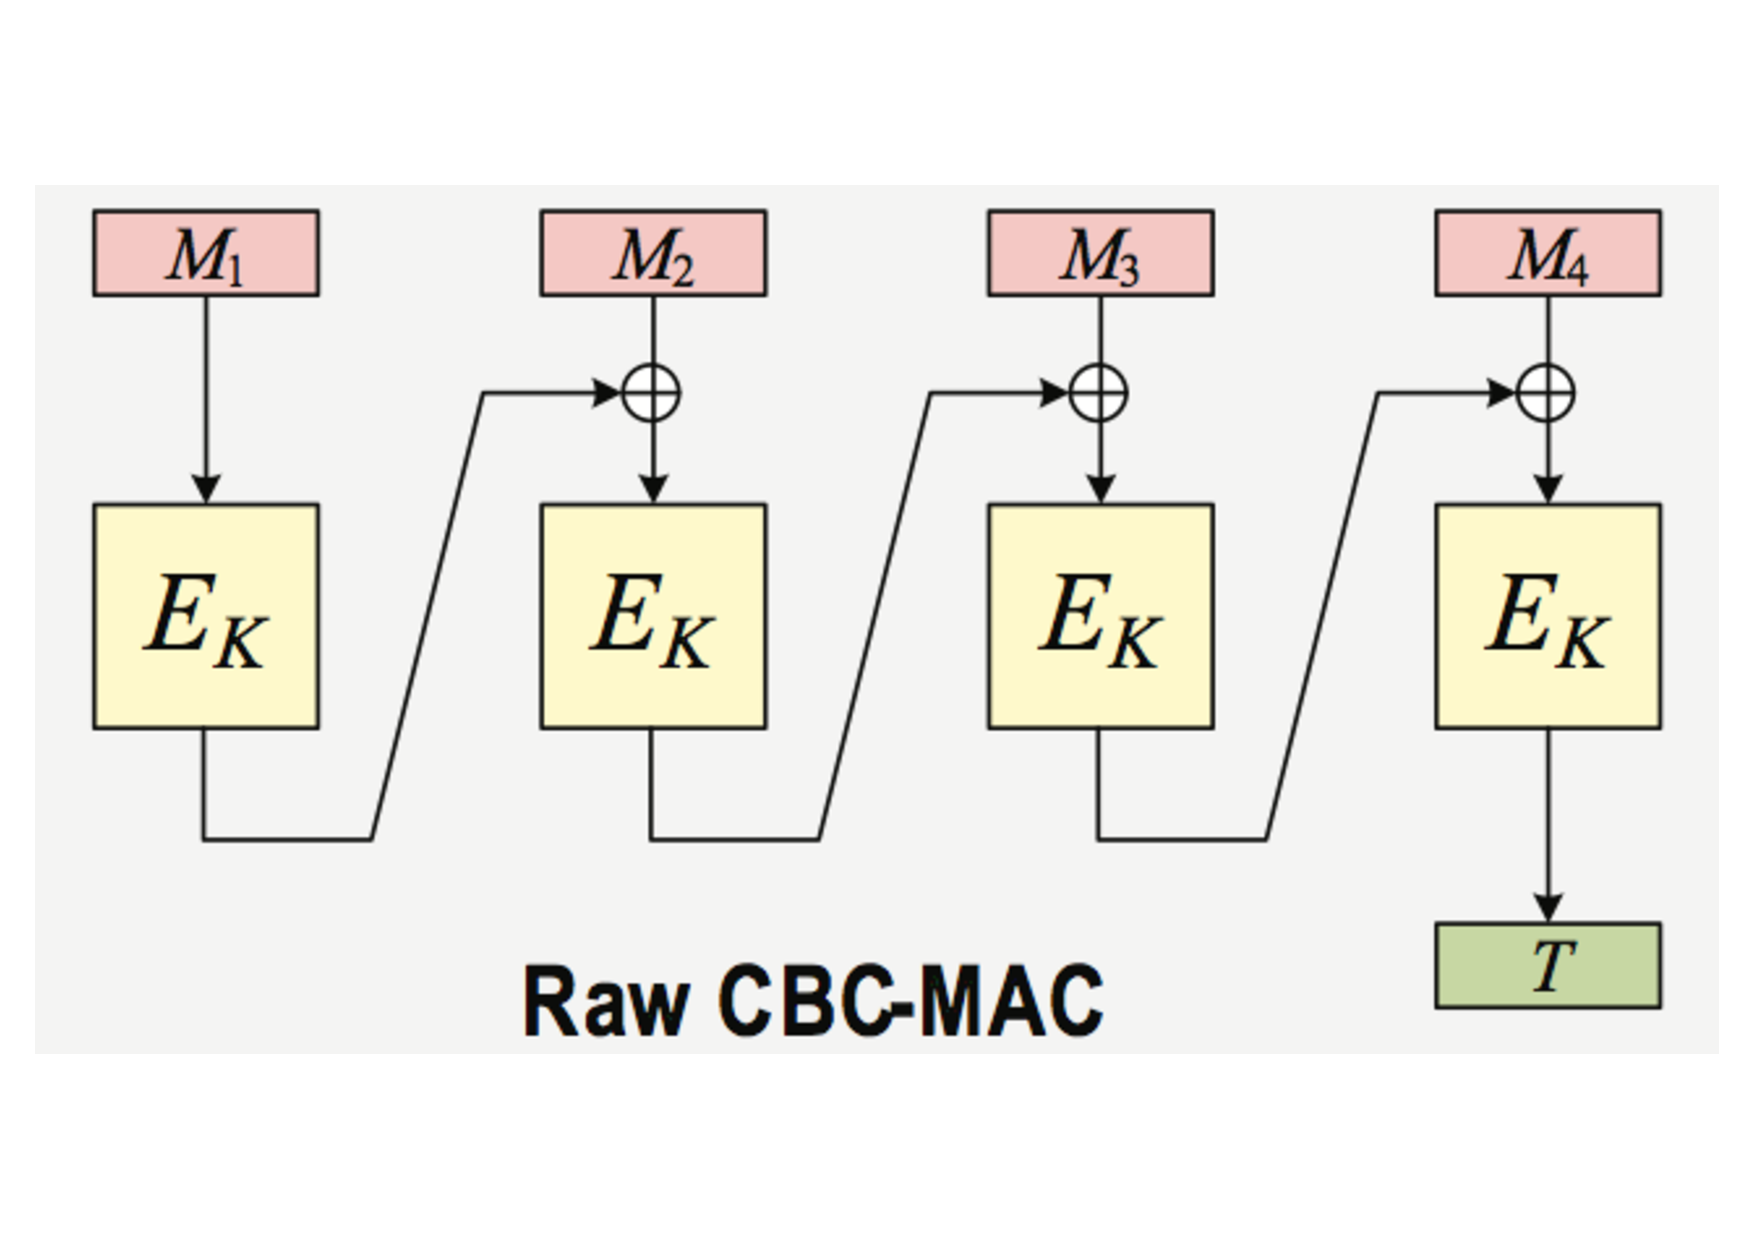
\includegraphics[scale=0.3]{./diagrams/cbc-mac.pdf}
\caption{The Raw CBC-MAC}
\label{CBC-mac }
\end{figure}
The research on iterated MAC schemes started from the raw CBC-MAC expressed in Figure 3.
\paragraph{Raw CBC-MAC}
The cryptographic primitive used in the raw CBC-MAC scheme is block cipher.  
The raw CBC-MAC is a secure MAC for only fixed length inputs. Assume the tag T of message M from CBC-MAC can be expressed as T = CBC-MAC$_k$(M), for another input M$\|$(M$\oplus$T), the tag T1=CBC-MAC(M$\|$(M$\oplus$T))=T. This attack indicates that the raw CBC-MAC is vulnerable if the input length is not fixed.
Besides the vulnerability when the input length is not fixed, the raw CBC-MAC scheme suffers birthday attack, means the adversary needs only 2$n/2$ input queries to succeed a forgery. 

Bellare et al. provided the original security evaluation on raw CBC-MAC\cite{cbc1994}. The conclusion is that if the adversary A is allowed to conduct arbitrary fixed length queries for q time, the probability that A succeeds in a forgery after the queries can be expressed with the queries times q and the computational assumption of block cipher used. Their quantitative conclusion showed that the forgery probability is very small.
\paragraph{EMAC}
The motivation of EMAC design is the problem that the raw CBC-MAC is secure only for fixed length inputs. 
EMAC is a optimized version of raw CBC-MAC providing security for arbitrary length inputs. The in the EMAC scheme, the final message block in the input is processed by a padding function to ensure that all the input blocks have the same length. Then raw CBC-MAC is applied applies and the result is encrypted by a the same block cipher in raw CBC-MAC with a different key. 

Petrank and Rackof provided the original security evaluation of EMAC in \cite{emac}. The EMAC is secure for arbitrary length inputs under the security notion if the block cipher meets the related computational assumptions. However, the EMAC still suffers the birthday attack.
\begin{figure}[htbp]
\centering
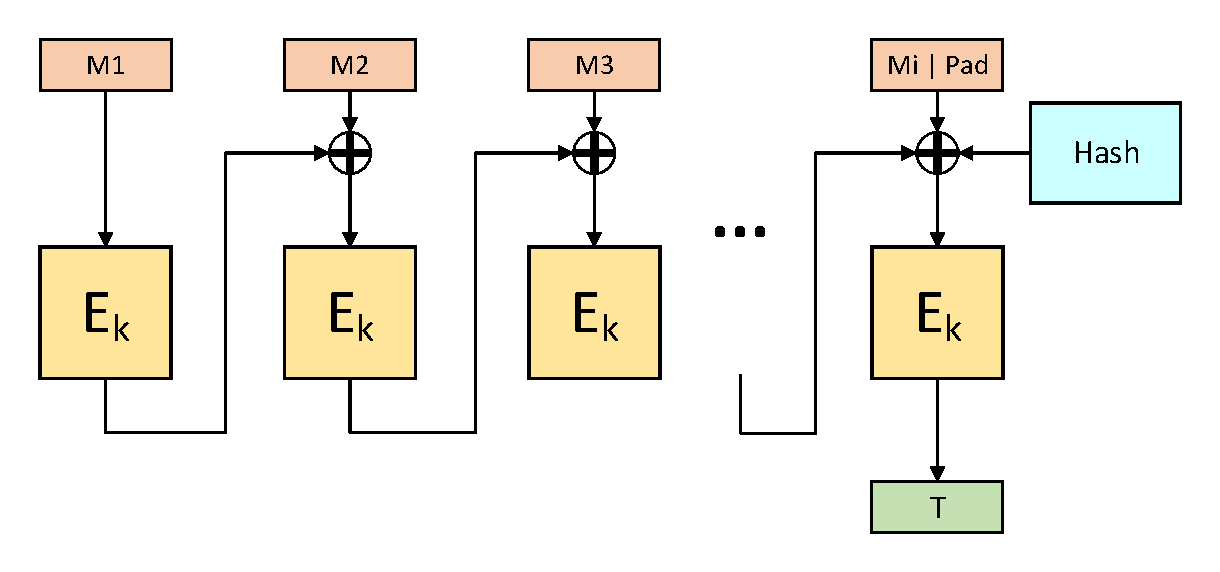
\includegraphics[scale=0.5]{./diagrams/cmac.pdf}
\caption{The class of CMAC}
\label{CMAC }
\end{figure}
Hence the raw CBC-MAC is vulnerable if the input length is not fixed, a class of MAC schemes named CMAC are developed to provide security for arbitrary length of inputs. The structure of the  variants of CMAC is modeled in Figure 4.
\paragraph{XCBC: three key version of CMAC }
Black and Rogaway introduced a optimized version of EMAC called XCBC in \cite{xcbc}.
There are two motivations of XCBC scheme: providing security for arbitrary length input; eliminate unnecessary padding operation on the input blocks in EMAC.

The XCBC scheme is a refined version of original EMAC. The contributions of XCBC scheme compared with the EMAC are: extending the domain to full domain; the block ciphers used in processing m input blocks is m other than m+1 in EMAC; all the block cipher in XCBC share a same key, the additional two keys are used to do exclusively or operation with the final input block,this design has faster processing speed.   

Black and Rogaway provided a original security analysis based on computational approach of XCBC scheme in \cite{xcbc}. Their quantitative result was improved by Minematsu and Matsushima in \cite{new}. 
\paragraph{TMAC: two key version of CMAC}
Kurosawa and Iwata designed a optimized version of cmac requiring two different keys in \cite{tmac} named TMAC.  
The two different keys used in processing the final input blocks in XCBC are replaced by a keyed hash function with two distinct constants as inputs. This optimization aims to reduce the key cost. 

Kurosawa and Iwata provided an original security analysis on TMAC in \cite{tmac} showing that the same level of security was achieved by TMAC compared with XCBC. The original quantitative security conclusion of TMAC was improved by Minematsu and Matsushima in \cite{new}. 
\paragraph{OMAC: single key version of CMAC}
Iwata and Kurosawa introduced a optimization of original XCBC scheme with only one key, named OMAC in \cite{omac}. This key is used by the block cipher in the OMAC and the keyed hash function used in TMAC is replaced by a result of Galois field multiplication. OMAC is the variant of CMAC using the least number of keys. 

Iwata and Kurosawa provided an original security analysis on OMAC in \cite{omac}. This result have no optimized version yet.
\paragraph{other iterated MAC designs}
Daemen and Rijmen introduced a iterated MAC design named ALRED-MAC in \cite{alred}. The motivation of of this work is the limitation of quantitative security result for iterated MAC scheme due to the birthday paradox. 
\paragraph{Parallel MAC Schemes}
The motivation of designing MAC schemes in which input message blocks are processed in parallel is the latency of processing when using iterated MAC schemes. This latency becomes more obvious when run the scheme on processors supporting pipeline of parallelism. 
In parallel MAC scheme, all the blocks in message M are processed in parallel. The output blocks of M processing are transformed to a single block B, then processed to generate tag T. 
\paragraph{XOR MAC scheme}
Bellare, Guerin and Rogaway introduced a parallel MAC scheme named XOR MAC in \cite{xor-mac}. 
The parallel input processing makes the xor MAC faster the CBC-MAC. 
In \cite{xor-mac}, the authors provided a quantitative security conclusion of xor mac that it is security under the security notion of message authentication system if the pseudorandom function used in the design is secure. The security bound of xor mac from \cite{xor-mac} expressed a smaller result compared with the result of raw CBC-MAC. 

The main weakness of XOR mac is the cost of storage for additional input parameters. According the design of XOR mac, assume the input message is divided into m blocks and the length of each block is half of the length of block cipher input. Each input block has a index with domain as [1,m]. A input block is the concatenated with the encoder of its index(whose length is same as the input block) to form the input to a block cipher, for example (i$\|$M[i]). Besides the m concatenated input blocks, a nonce formed with random number or counter is used a input to the block cipher. Then the m+1 output blocks from block cipher is xored and the output block of XOR operation is concatenated with a random number or counter to form the final tag. 
We can see that the length of tag from XOR-mac is the sum of the length of a output block from block cipher and the length of a random number or counter. This long-length MAC needs additional storage compared with the tag from iterated MAC schemes. 
On the other hand, the nonce maintained by the user of XOR mac is regarded a disadvantage by some researchers.
\begin{figure}[htbp]
\centering
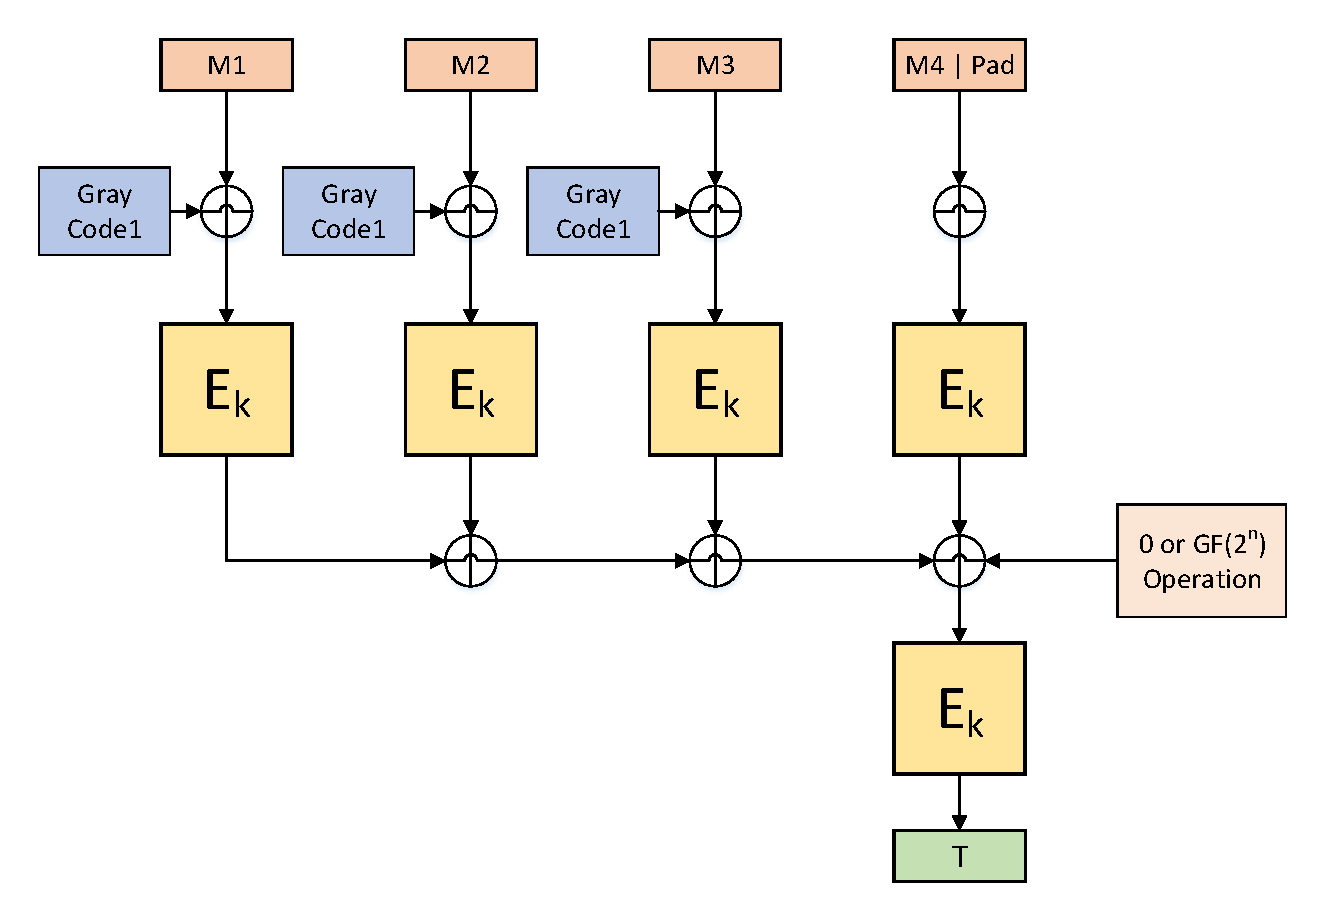
\includegraphics[scale=0.5]{./diagrams/PMAC.pdf}
\caption{RAW PMAC}
\label{PMAC}
\end{figure}
\paragraph{Raw PMAC}
Black and Rogaway introduced an parallel MAC scheme named PMAC in \cite{pmac}. 
The improvement of PMAC compared with XOR MAC is the less calling of block cipher when generating a tag. Secondly, there is no limitation for the input length when using PMAC. 
Another benefit brought by PMAC is that only one key is needed in generating the tag. Other processing operations include bit-level xor and gray code, which are cost-effective and fast processing. 

The quantitative security result of PMAC was acquired by Black and Rogaway in \cite{pmac}. They analysed the probability of internal collision in the arbitrary types of inputs and asserted that the PMAC design is a secure MAC if the block cipher used behaves like a pseudorandom permutation. In the proof from Black and Rogaway, the probability that an adversary can distinguish the PMAC from pseudorandom function is the probability that collision of internal blocks(the outputs of block cipher) plus the probability of tag collision. 

Lee et al. posted attacks on the raw PMAC in \cite{pmac_forgery}. Their research indicated that the raw PMAC design did not bring advantage in security compared with iterated MACs. The raw PMAC suffers from their birthday like attack and the key recover attack.
\paragraph{Tweakable block cipher and Optimized PMAC}
The concept of tweakable block cipher was formally defined by Liskov, Rivest, and Wagner in \cite{tweak}. Rogaway introduced a efficient implementation of tweakable block cipher in \cite{tweak_pmac}and adopt this implementation to replace the block cipher used in the original PMAC and OCB authenticated encryption mode.
The application of tweakable block cipher in constructing PMAC can enhance the processing speed compared with original PMAC based on Grey code and simplify the structure of the scheme, which also simplify the security analysis of the scheme. 

In \cite{tweak_pmac}, Rogaway provided an assertion that the tweakable block cipher XE and XEX behave like a pseudorandom permutation if the block cipher inside is a pseudorandom permutation. Based on this assertion about security of tweakable block cipher, Rogaway gave an quantitative conclusion that the new PMAC based on tweakable block cipher is security under the security notion of message authentication system. This quantitative security result of tweakable block cipher based PMAC was provided in \cite{tweak_pmac}.
Minematsu and Matsushima optimized this result in \cite{new}. 

The evaluation procedure in \cite{pmac} is questioned by the latter researchers hence the correlation between collision probability and 
distinguishing probability was not explained . This issue was also pointed in Nandi`s improved analysis on PMAC in \cite{improve_pmac}. Nandi also provided a improved quantitative security result of PMAC which is smaller in all the cases than the one in \cite{pmac} and \cite{new}. 
\paragraph{iPMAC}
Sarkar introduce an optimisation on original PMAC in \cite{iPMAC}. The galois field multiplication used in the tweakable block cipher introduced is replaced by a technique named tower field representation of Galois field. This replacement enhance the processing speed in software.

Hence the structure of iPMAC is same as the original PMAC except the input masking stage, the security evaluation by the author in \cite{iPMAC} followed the approach in \cite{pmac}.

\subsubsection{Stateful MAC Schemes}
Deterministic MAC schemes cannot defend against the second type of attack in the
threat model defined in Section 2 . The reason is that the secrete key used in generating the tag will not be refreshed for each message. If two message are identical, their tags are identical. To address this issue, nonce is introduced to the tag generation in a MAC scheme. A nonce is a short message block whose value will be updated by each message in tag generation. To update the value of nonce, the address of message, a random number, a counter or the combination of these three elements are adopted in the nonce generation for each message. With the nonce introduced, a well designed stately MAC scheme should be capable in defending type 2 attack in threat model.
\paragraph{GMAC}
McGrew and Viega introduced the Galois/Counter Mode authenticated encryption design and the original security analysis is provided in \cite{gcm}. The message authentication system in GCM(named GMAC) is a iterated scheme based on the concept of universal hashing. The block processing component used in GMAC is the Galois field multiplication other than the block cipher in deterministic MAC schemes. 
The motivation of GCM is to design a scheme combining counter mode of operation(CTR) with a message authentication code(the GMAC) to form a efficient and secure authenticated encryption system.
One advantage of adopting the Galois field multiplication in GMAC is that it can be made easily in hardware and has efficient performance in software. 

In the security analysis of GCM from McGrew and Viega, the GMAC was not discussed alone. The security of GMAC as a message authentication code is based on the fact that the encryption part in GCM is secure and the collision probability of ciphertext blocks is low. 
In GCM design, the nonce is called initialization vector (IV). For each invocation of GCM, the IV should be distinct.

In \cite{breaking}, Iwata, Ohashi and Minematsu provided an optimised analysis for the security of GCM. They pointed out the weakness in the lemma used in forming the bound of the quantitative result of security for GCM with a counter example. This counter example was developed to a distinguishing attack on GCM. Iwata et al. then provided a approach fixing the problem of original lemma and provided the new quantitative security result of GCM. 

In \cite{Rogaway2011}, Rogaway pointed the weakness of GMAC as a MAC scheme when used alone that the security under adaptive chosen-message attack is not as good as the security of deterministic MAC schemes. On the other hand, GMAC requires the nonce for tag generation and this nonce should be maintained and refreshed by the user of GMAC. The potential issue of this design pointed by Rogaway is the reuse of nonce, which may lead to the collision of the tag. 

Handschuh and Preneel introduced key-recovery attacks on universal hash function based MAC algorithms in \cite{key_recover}. They introduced two types of attacks: weak key finding and partial information leaks.

\subsection{Authentication-Ecryption Schemes and Security Analysis}
After various kind of MAC schemes were evaluated and claimed to be secure, a new cryptosystem, the Authenticated Encryption(AE) was introduced The Authenticated to combine the encryption of
plaintext blocks and generation of the MAC in a single scheme to provide both
confidentiality and integrity. According to the analysis of by Bellare and Namprempre in \cite{ae-notion}, AE schemes can be categorized as Encrypt-then-MAC, Encrypt-and-MAC and MAC-then-Encrypt three structures. Encrypt-then-MAC was proved to be most secure structure and can defend most kinds of attacks. 
In Rogawa`s works \cite{aead} a systematical analysis about AE
schemes using associate data was expressed.  

Based the notion of security evaluation for AE systems introduced in \cite{aead}, the security of several AE schemes in
Encrypt-then-MAC mode have been analyzed systematically, including CCM \cite{ccm}based on
CBC-MAC,EAX\cite{eax} based on OMAC, GCM
\cite{gcm} based on universal hashing(new bound revised in \cite{breaking}), and
OCB\cite{ocb} based on PMAC(new bound revised in \cite{tweak,iPMAC}). Kasper and
Schwabe introduced a implementation of AES that run faster than previous AES block cipher
and adopted this implementation to construct a faster AES-GCM AE
scheme\cite{fast}.
\paragraph{Attacking the Authentication Systems}
There were research works on attacks to existing authentication system or AE systems, such as
\cite{cycle,attack_blk,hardware_attack}. Some of these works recover the security weakness in the design works while some other works depict attacks that are out of the security bound of system analyzed. 

\subsection{Hardware Message Authentication(MA) Systems}
\paragraph{Concepts of Message Authentication(MA) System}
After various kinds of MAC schemes and authenticated-encryption schemes are evaluated systematically, researchers have paid effort on designing Message Authentication(MA) system to protect data integrity from or to the cache on-chip. 
In the design of Message Authentication(MA) system, the on-chip data is assumed to be inaccessible and secure, and the chip is called trusted area; while the data in the transmission and stored in off-chip memory is considered to be accessible to attackers and vulnerable. Transmission path(such as bus) and off-chip memory are called malicious area. 
\begin{figure}[htbp]
\centering
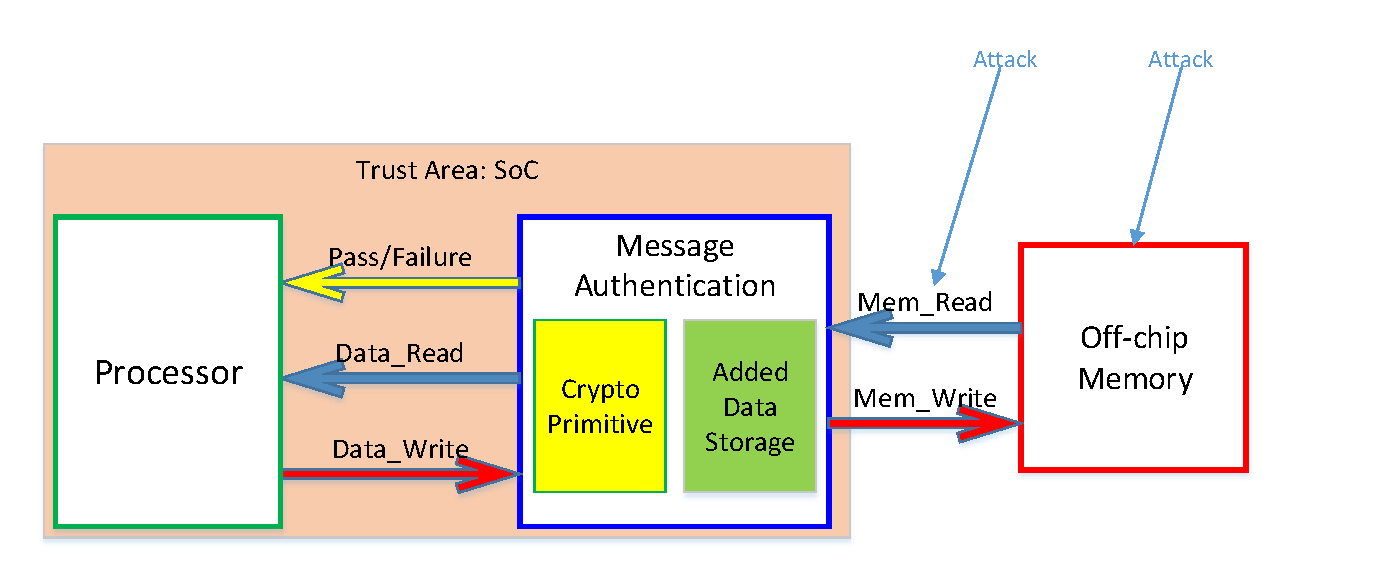
\includegraphics[scale=0.5]{./diagrams/MA_concept.pdf}
\caption{The Concept of MA System}
\label{ma_system}
\end{figure}
Figure 1 expresses the concept of MA system for chip-memory communication. 
When processor writes a data block, marked as D, to and address, marked as addr, on the memory, processor sends D to MA system and output a message block, marked as message(D, add$_B$), where add$_B$ represents an additional data block. The message block message(D,add$_B$) can be the data block D only, D concatenated with a short block(commonly called tag) or other format of D. The content of message(D,add$_B$) is determined by the cryptographic primitive adopted by the MA system.
When the processor wants to read the data D from address addr, the message(D,add$_B$) is read to SoC and sent to MA system first. After verified by MA, if the data D is not tampered, MA sends a signal indicating pass to processor and send the D to the processor, where D is extracted from message(D,add$_B$) block read from memory.
If the MA system finds that the D is tampered, MA sends a failure signal to processor, and invoke the exception handling procedure.
\paragraph{Security Evaluation for MA Systems}
As discussed with previous articles, encryption can only protect the integrity of data from and to the cache. Authentication Primitives(AP) should be adopted on the chip to process the data with additional information block, such as secret key or nonce. 

The processed data will be transfered to the off-chip area in a specific message format. The message is ciphertext blocks for hash function, [ciphertext $\mid$ tag] for MAC scheme, and E$_k$[plaintext $\mid$ nonce] for AREA. The first step to evaluate the security of a MA system is figure out the AP system adopted and additional information needed. 

For each kind of AP design, there are requirements on the inputs to the AP system. For example, a MAC scheme accepting a nonce requires the nonce to be distinct to each data that invoke the MAC scheme. This requirement ensure that the scheme can defend two types of attacks in the threat model. The MA system design based on such a MAC scheme should ensure that for each data write to the off-chip area from cache, the related nonce should be distinctive. Otherwise, the MA system design is not secure. The second step in security evaluation on a MA system is figure out whether the requirements on inputs of AP system is met.

If the MA system design meets the requirements of inputs for the AP system adopted, it is necessary to figure out what information is stored in off-chip area and what else are on-chip. Using MAC scheme as instance, the nonce and secrete key in tag generation should be inaccessible to the attacker.  
The third step to evaluation the security of an MA system is examine the information stored on-chip and off-chip. If there is some information that can be adopted by the attacker to break the authentication system, the MA design can be assume not secure.

The fourth step to evaluate the security of a MA system is analyzing the security of AP adopted. If the AP system is a novel design without previous systematically analysis, it is necessary to do the analysis with a evaluation mechanism, such as computational model based on provable security theory.

The final step is drawing the conclusion of the security of MA system. If the system does not fail in any one of previous four steps, the MA system is secure in general security notions and can effectively defend some kind of attacks.

Some MA systems are constructed based on authenticated-encryption schemes to
provide protection on both confidentiality and integrity of data. 
\paragraph{Uni-processor Systems}
In \cite{yan-MA}, Yan et al. proposed a MA design based on a variant of Galois/Counter Mode(GCM) authenticated encryption scheme proposed by McGrew and Viega in \cite{gcm}. A data block to be protected is spliced to several chunks each of whose length is same as the length of input to block cipher. For each chunk, a tuple(address, counter, random value(EIV)) is generated as chunk nonce for encryption. For the whole data block, a tuple (address of chunk 1, counter, random value 2(AIV)) is generated for tag generation. 
In the design from Yan et al., the counter for a data block is formed by two parts: a long-length major counter(64 bits) concatenated with a short-length minor counter(no more than 8 bits). When the minor counter overflow, the major counter updates. For each data block, the counter is distinct. For each chunk in a data block, the address is distinct and the counter is same. The frequency of updating EIV depends on the security level required by the whole system.  In this way, the nonce for each chunk and the whole data block is update for each invocation of GCM scheme. As the security of GCM scheme has been systematically analyzed in \cite{gcm} and the security result was optimized by Iwata, Ohashi and Minematsu in \cite{breaking}, the design from Yan et al. is a secure design.


In \cite{pc-ice}, Elbaz et al. introduced a hardware design aiming to protect both the confidentiality and integrity of data. The structure adopted in this design is similar to MAC-then-Encrypt. The tag for read-only data is the address of the data, while the tag for read-write data is the address of data concatenated with a random number. Data protected is concatenated with the tag and encrypted with block cipher. The ciphertext block is sent to off-chip area.
One weakness of this design is that MAC-then-Encrypt is less secure compared with Encrypt-then-MAC structure as MAC-then-Encrypt can not defend NM-CPA attack. This proposition was proved by Bellare and Namprempre in \cite{ae-notion}.
Another weakness of security is that the bit-length of random number in the tag design is short, which is easy to collide if the amount of data to protect is large. The easy-to-collide tag can enhance the probability of succeed for the attacker.


In \cite{rogers-MA} Rogers and Milenkovic proposed an AE system design aiming to offer protection on confidentiality and integrity of both code and data. In this design, the protection mechanism for static data is same as the one for code while the mechanism for dynamic data is different.
The structure of AE scheme adopted in the design from Rogers and Milenkovic is Encrypt-and-MAC. The MAC scheme adopted is a variant of PMAC. When using this variant to generate a tag for the data protected, the addressed and a unique sequence number are introduced as additional information aiming to defend type 2 attack in the threat model. The sequence number is unique to each data that invoke the tag generation.
One weakness of the design from Rogers et al. is that Encrypt-and-MAC structure is less secure according to the analysis from Bellare and Namprempre in \cite{ae-notion}. On the other hand, there is two distinct secret keys adopted in the tag generation, which introduce additional on-chip cost.

In \cite{vaslin-MA}, Vaslin et al. designed an AE system using one-time pad(OTP) for encryption and CRC checksum module for integrity checking. For each data protected, a tuple(address, timestamp(TS), padding value(PV)) is encrypted to form a OTP. A checksum is computed with CRC using plaintext data as input. This checksum is stored on-chip. The timestamp for each data is also recored on the chip. The OTP is xored with plaintext data to form the ciphertext. The ciphertext is sent to off-chip area. 
When cache reads data, ciphertext block is read to chip, xored with the OTP computed with tuple(address, timestamp(TS), PV). The output of xor is used to compute a checksum(CS2) with CRC and compared to the checksum(CS1) on-chip. 
The weakness of this design is that CRC is less secure compared with hash functions such as MD5 or SHA-1. This weakness was pointed by the authors in this paper and by Elbaz et al. in \cite{area}.

\bibliographystyle{plain}
\bibliography{./resources/tag_paper.bib}
\end{document}
